\documentclass{article}

\usepackage{color}
\usepackage{tikz}
\usepackage{float}
\usepackage{tabularx}
\usepackage{amsmath}
\usepackage{amssymb}
\usepackage{listings}
\usepackage{enumitem}
\usepackage{syntax}
\usepackage{csquotes}
\usepackage{pgfplots}
\usepackage{parskip}
\usepackage{fancyhdr}
\usepackage{vmargin}
%\usepackage[backend=biber]{biblatex}
%\addbibresource{references.bib}


\definecolor{dkgreen}{rgb}{0,0.6,0}
\definecolor{gray}{rgb}{0.5,0.5,0.5}
\definecolor{mauve}{rgb}{0.58,0,0.82}

% Plots
\usepackage{pgfplots}
\usepackage{pgfplotstable}
\pgfplotsset{filter discard warning=false}
\pgfplotsset{
    discard if/.style 2 args={
        x filter/.append code={
            \edef\tempa{\thisrow{#1}}
            \edef\tempb{#2}
            \ifx\tempa\tempb
                \def\pgfmathresult{inf}
            \fi
        }
    },
    discard if not/.style 2 args={
        x filter/.append code={
            \edef\tempa{\thisrow{#1}}
            \edef\tempb{#2}
            \ifx\tempa\tempb
            \else
                \def\pgfmathresult{inf}
            \fi
        }
    },
    discard if smaller/.style n args={2}{
    	x filter/.code={
            \edef\tempa{\thisrow{#1}}
            \edef\tempb{#2}
                \ifnum\tempa<\tempb
                    \def\pgfmathresult{inf}
                \else
                \fi
        }
    },
    discard if larger/.style n args={2}{
    	x filter/.code={
            \edef\tempa{\thisrow{#1}}
            \edef\tempb{#2}
                \ifnum\tempa>\tempb
                    \def\pgfmathresult{inf}
                \else
                \fi
        }
    }
}


% Listings
\usepackage{algorithm}
\usepackage[noend]{algpseudocode}

\lstset{frame=tb,
  numbers=left,
  stepnumber=1,
  language=Java,
  aboveskip=3mm,
  belowskip=3mm,
  showstringspaces=false,
  columns=flexible,
  basicstyle={\small\ttfamily},
  numberstyle=\color{gray},
  keywordstyle=\color{blue},
  commentstyle=\color{dkgreen},
  stringstyle=\color{mauve},
  breaklines=true,
  breakatwhitespace=true,
  tabsize=2,
  moredelim=**[is][\color{red}]{@}{@},
}

\setlength{\grammarindent}{12em}

%\renewcommand{\lstlistingname}{Algorithm}
%\newcommand{\tablerow}[4]{ #1 & #2 & #3 & #4\\}
\newcommand{\n}[0]{\\[\baselineskip]}

% TITLE PAGE
% #1 - Module code
% #2 - Lecturer
\newcommand{\maketitlepage}[2]{
\begin{titlepage}
	\centering
    
\includegraphics[scale = 0.4]{imgs/logo.png}\\	% University Logo
	\textsc{\LARGE #1}\\[0.5 cm]				% Course Code
	\rule{\linewidth}{0.2 mm} \\[0.4 cm]
	{ \huge \bfseries \thetitle}
	\rule{\linewidth}{0.2 mm} \\[0.5 cm]
	\textsc{\large \thedate}\\[1.5 cm]
	
	\begin{minipage}{0.4\textwidth}
		\begin{flushleft} \large
			\emph{Lecturer:}\\
			#2
			\end{flushleft}
			\end{minipage}~
			\begin{minipage}{0.4\textwidth}
            
			\begin{flushright} \large
			\emph{Submitted By:} \\
			\theauthor
		\end{flushright}
        
	\end{minipage}\\[2 cm]
	
\end{titlepage}
}




\title{Classification of object colour using optical spectroscopy}
\author{140011146}

\makeatletter
\let\thetitle\@title
\let\theauthor\@author
\let\thedate\@date
\makeatother

\begin{document}

\maketitlepage{CS5014 Machine Learning}{David Harris-Birtill\\Kasim Terzi\'{c}}




\section{Introduction}

In this practical, two classification tasks were performed on an experimental dataset. 

\section{Binary Classification}

\subsection{Preprocessing}
Before any preprocessing is done, the data was split into training and test datasets. This is to ensure no bias when looking at the data, even for visualisations. 


\subsubsection{Data visualisation}
First, the spectroscopy data can be visualised by plotting the intensities and wavelengths to see if there are visual patterns than can be seen in the data. As there are over nine hundred input features, it is likely many of them are either redundant or not well correlated to the input data. 

\begin{figure}[H]
\centering
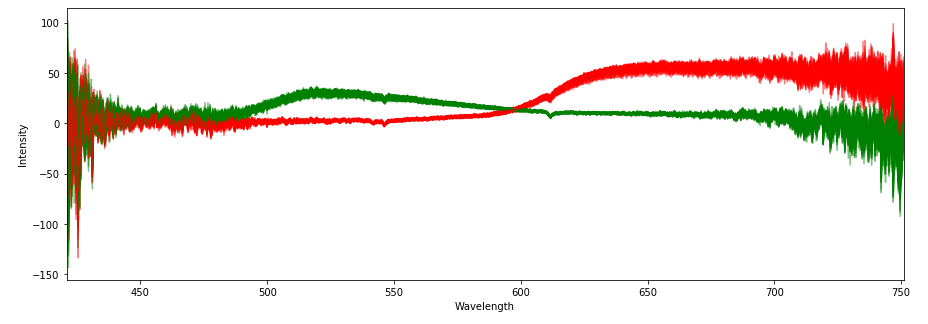
\includegraphics[width=1\textwidth, keepaspectratio]{imgs/binary-visual.png}
\caption{Initial plot of the data, showing the intensity of the wavelengths measured. The plot is colour coded with the output so any differences between the red and green data can be easily seen.}
\label{fig:binary-visual}
\end{figure}
\noindent
From the visualisation, it is interesting to see that for many wavelengths, there is a very clear distinction between the red and green intensities. This suggests that for those wavelengths, it would be very simple to classify. Further, the visualisation was created from all the training data, so it can be seen there are no large errors in the middle wavelengths where no data points incurred significant differences, which shows the consistency of the data. It can be see towards the start and end of the spectrum, the intensities are more varied, indicating possible errors during measurement. As such, it would make sense when choosing input features to mostly include features from the middle wavelengths where less possible errors occurred. 

\subsubsection{Data correlation}
Next, the correlation of each input feature wavelength can be calculated and plotted to see how the set of input features is correlated to the output. 
\begin{figure}[H]
\centering
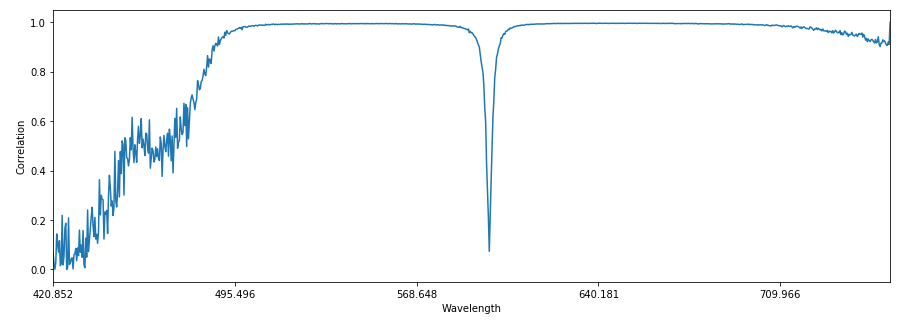
\includegraphics[width=1\textwidth, keepaspectratio]{imgs/binary-correlation.png}
\caption{Correlation of each wavelength input feature to the output classification.}
\label{fig:binary-correlation}
\end{figure}
\noindent
The curve of input feature correlation corresponds very closely to figure \ref{fig:binary-visual}. At the wavelengths where the red and green curves become distinct from each other, the correlation of that wavelength to the output class tends to perfect correlation. At the center where the red and green curves cross over, a dip in the correlation can be seen as it becomes difficult to distinguish the two in the overlap. 

\subsection{Results}

\begin{figure}[H]
\centering
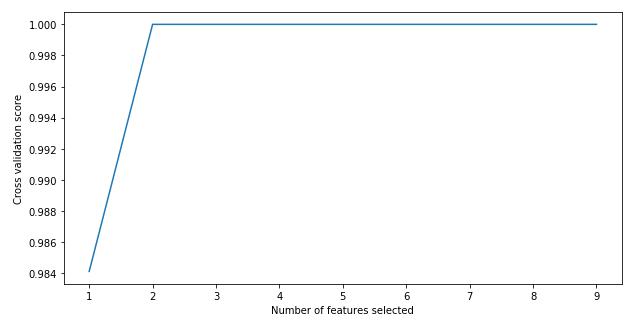
\includegraphics[width=1\textwidth, keepaspectratio]{imgs/binary-numfeatures.png}
\caption{Cross validation accuracy score of increasing number of features using recursive feature elimination.}
\end{figure}

\section{Multiclass Classification}

\subsection{Preprocessing}

\subsubsection{Data visualisation}

\begin{figure}[H]
\centering
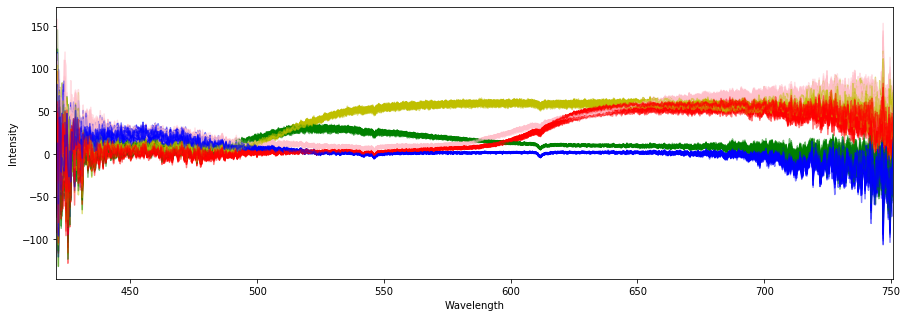
\includegraphics[width=1\textwidth, keepaspectratio]{imgs/multiclass-visual.png}
\caption{Plot of the data to show the intensity of wavelengths of the different colour classes.}
\end{figure}

\subsubsection{Data correlation}

\begin{figure}[H]
\centering
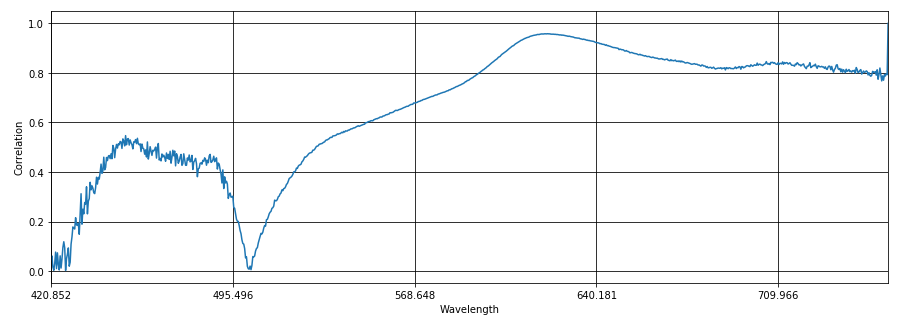
\includegraphics[width=1\textwidth, keepaspectratio]{imgs/multiclass-correlation.png}
\caption{Correlation of each wavelength input feature to the colour classification.}
\end{figure}

\subsection{Results}

\section{Conclusion and Evaluation}

%\printbibliography

\end{document}



